\section{Solving Laplace's Equation in Two Dimensions}
\label{sec:laplace}

Here Laplace's equation in two dimensions,
\begin{equation}
    \nabla^2 \varphi = 0,
\end{equation}
is solved using the finite difference equation given in Equation \ref{eqn:iteration} with $\rho = 0$. All non-boundary nodes are set to random guesses between 0 and 1 and the number of iterations is capped at \texttt{max\_it}$=10000$.

\subsection{Basic Verification}
\label{subsec:basic_verification}

The program has in-built boundary conditions for a parallel plate capacitor, a plane equipotential, a single point charge-like equipotential in the middle of the grid, a net with constant potential around the edges of the grid and a cross equipotential. The resulting solutions are plotted in Figures \ref{fig:plane}, \ref{fig:capacitor}, \ref{fig:point}, \ref{fig:net} and \ref{fig:cross}. These basic examples agree with visually with the analytic solutions\cite{gardner2013}. A more detailed analysis of the calculated solution to the Laplace equation around a parallel plate capacitor with a numerical comparison to the analytic solution can be found in Section \ref{subsec:infinite_plate_solution}.

\begin{figure}
    \centering
    \subfloat[Contour plot]{
        \includegraphics[width=0.3\linewidth]{graphs/examples/plane_contour.eps}
        \label{subfig:plane_cont}
    }
    \subfloat[Surface plot]{
        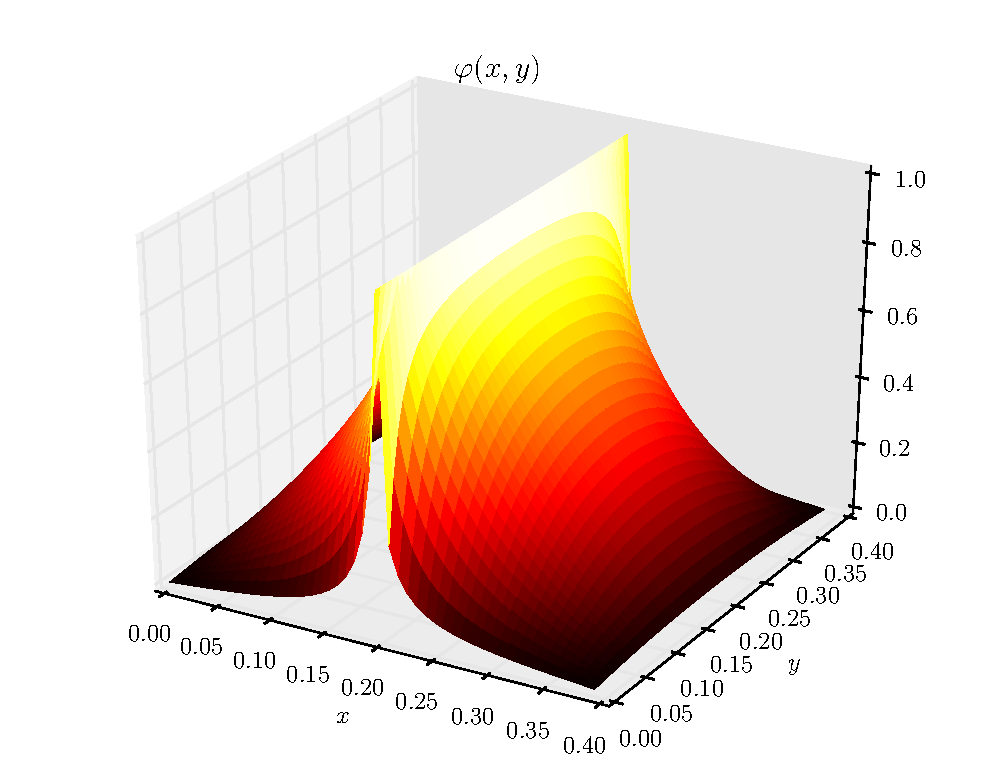
\includegraphics[width=0.3\linewidth]{graphs/examples/plane_surf.eps}
        \label{subfig:plane_surf}
    }
    \subfloat[Vector \textbf{E} field plot]{
        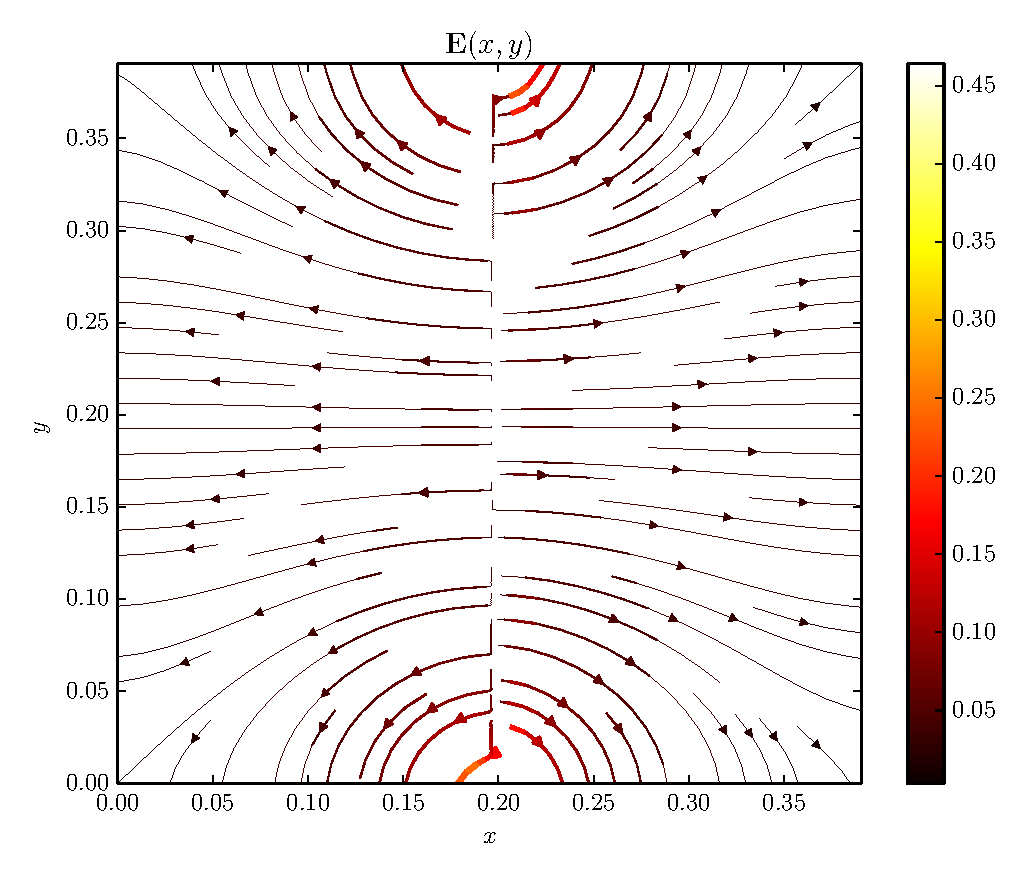
\includegraphics[width=0.3\linewidth]{graphs/examples/plane_vector.eps}
        \label{subfig:plane_vect}
    }
    \caption{Plots of the solution to the Laplace equation with boundary conditions of an equipotential plane.}
    \label{fig:plane}
\end{figure}

\begin{figure}
    \centering
    \subfloat[Contour plot]{
        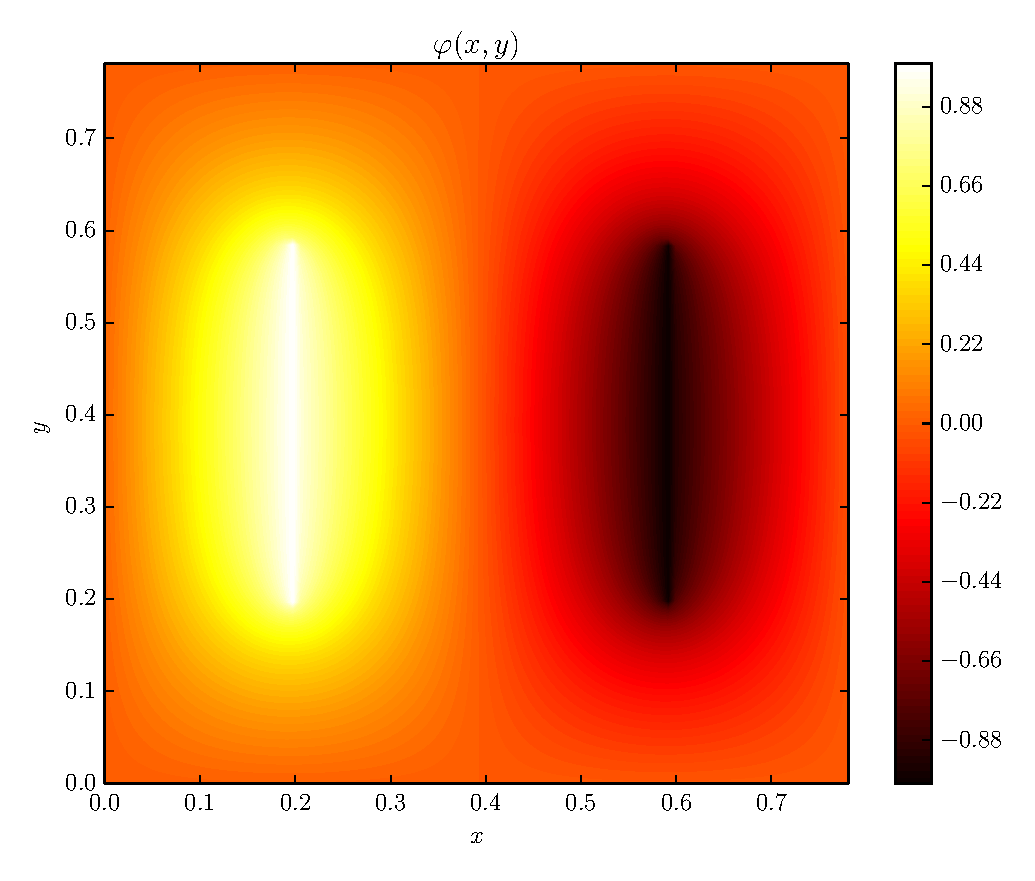
\includegraphics[width=0.3\linewidth]{graphs/examples/capacitor_contour.eps}
        \label{subfig:capacitor_cont}
    }
    \subfloat[Surface plot]{
        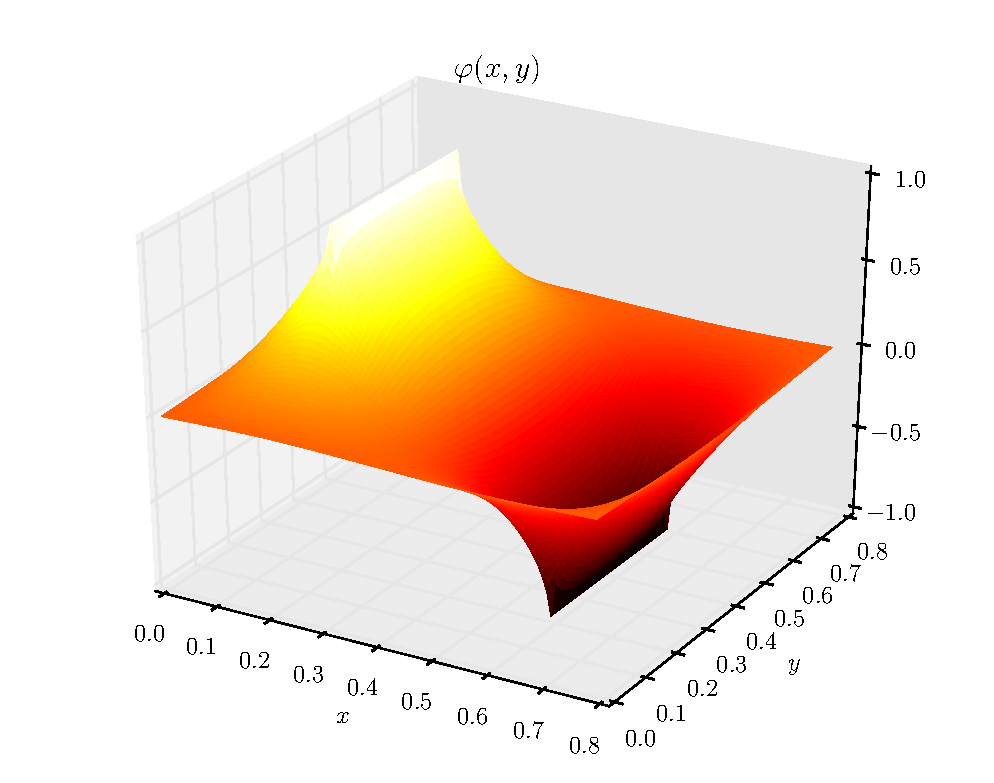
\includegraphics[width=0.3\linewidth]{graphs/examples/capacitor_surf.eps}
        \label{subfig:capacitor_surf}
    }
    \subfloat[Vector \textbf{E} field plot]{
        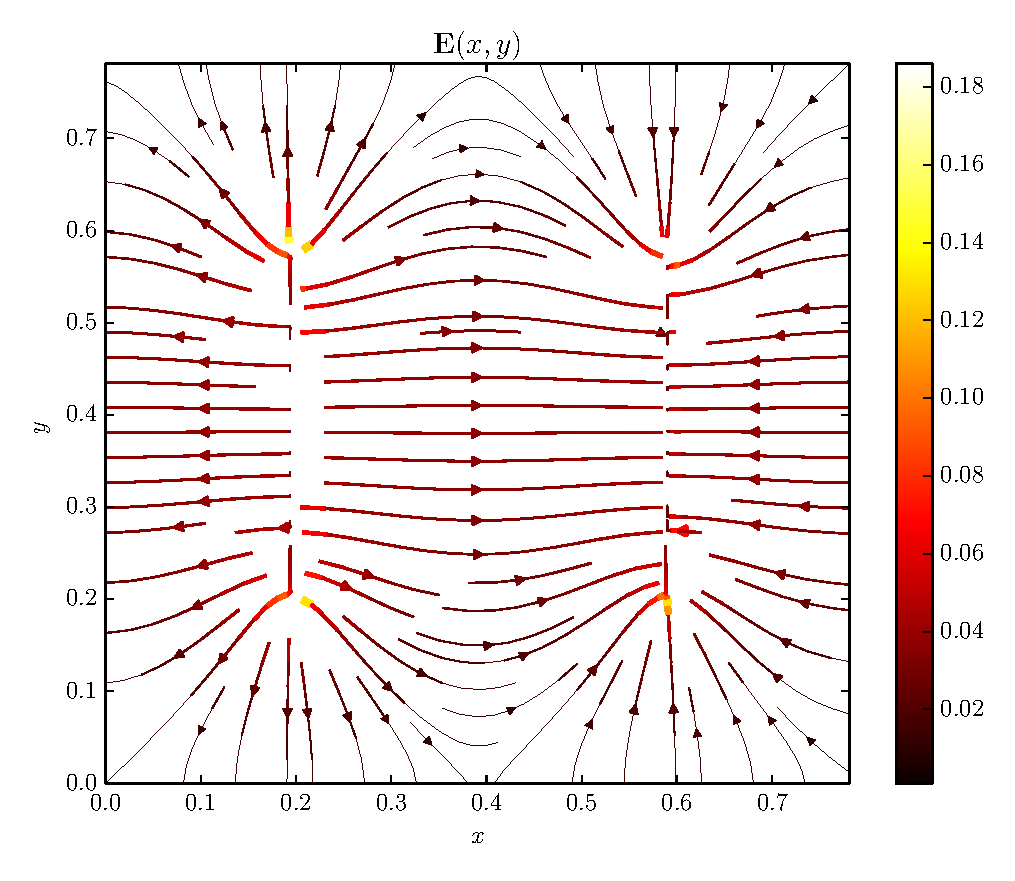
\includegraphics[width=0.3\linewidth]{graphs/examples/capacitor_vector.eps}
        \label{subfig:capacitor_vect}
    }
    \caption{Plots of the solution to the Laplace equation for a parallel plate capacitor.}
    \label{fig:capacitor}
\end{figure}

\begin{figure}
    \centering
    \subfloat[Contour plot]{
        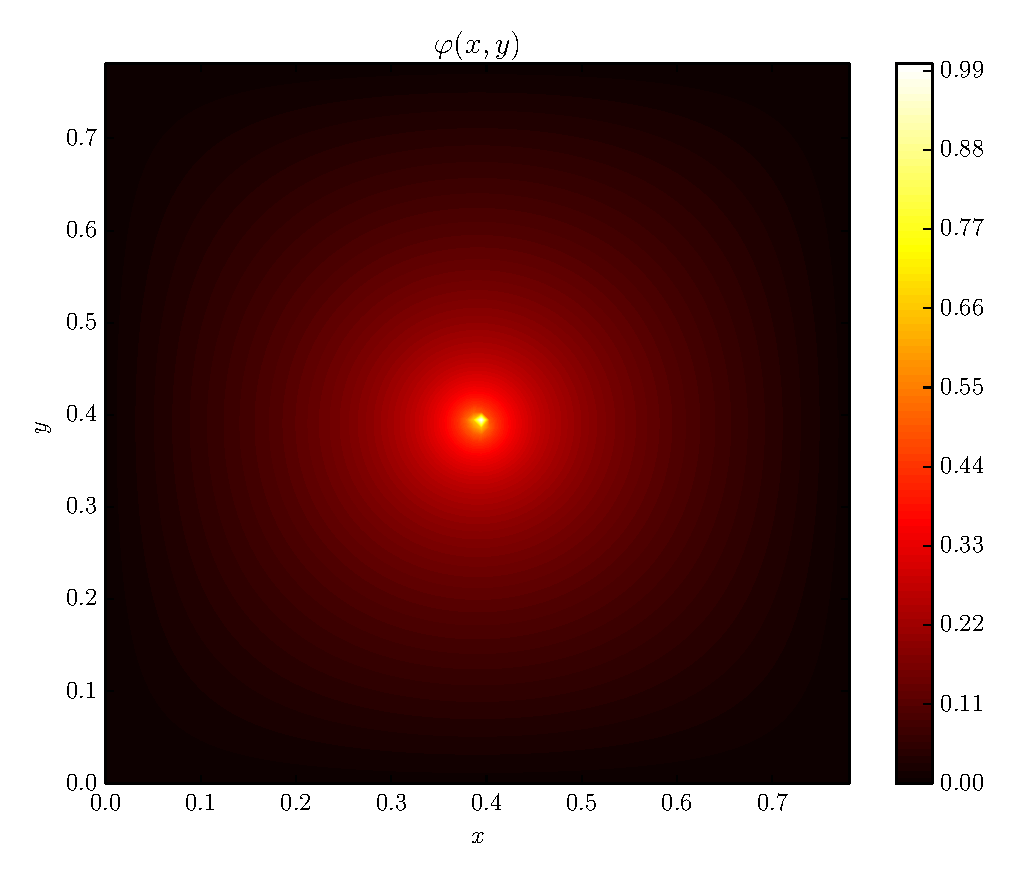
\includegraphics[width=0.3\linewidth]{graphs/examples/point_charge_contour.eps}
        \label{subfig:point_cont}
    }
    \subfloat[Surface plot]{
        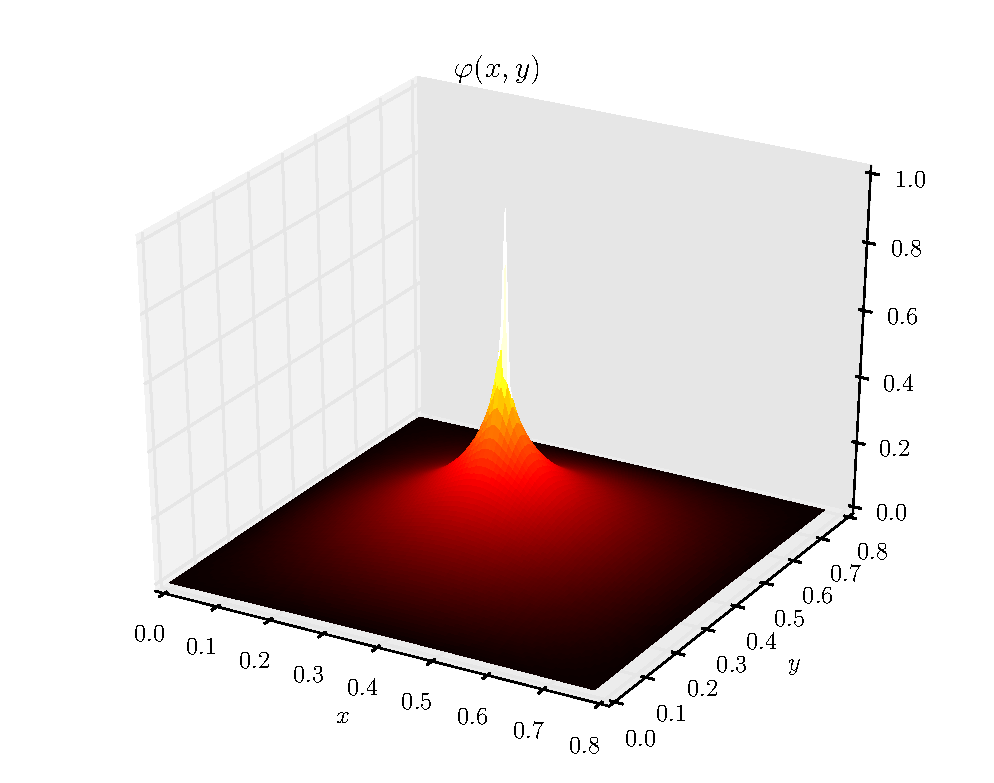
\includegraphics[width=0.3\linewidth]{graphs/examples/point_charge_surf.eps}
        \label{subfig:point_surf}
    }
    \subfloat[Vector \textbf{E} field plot]{
        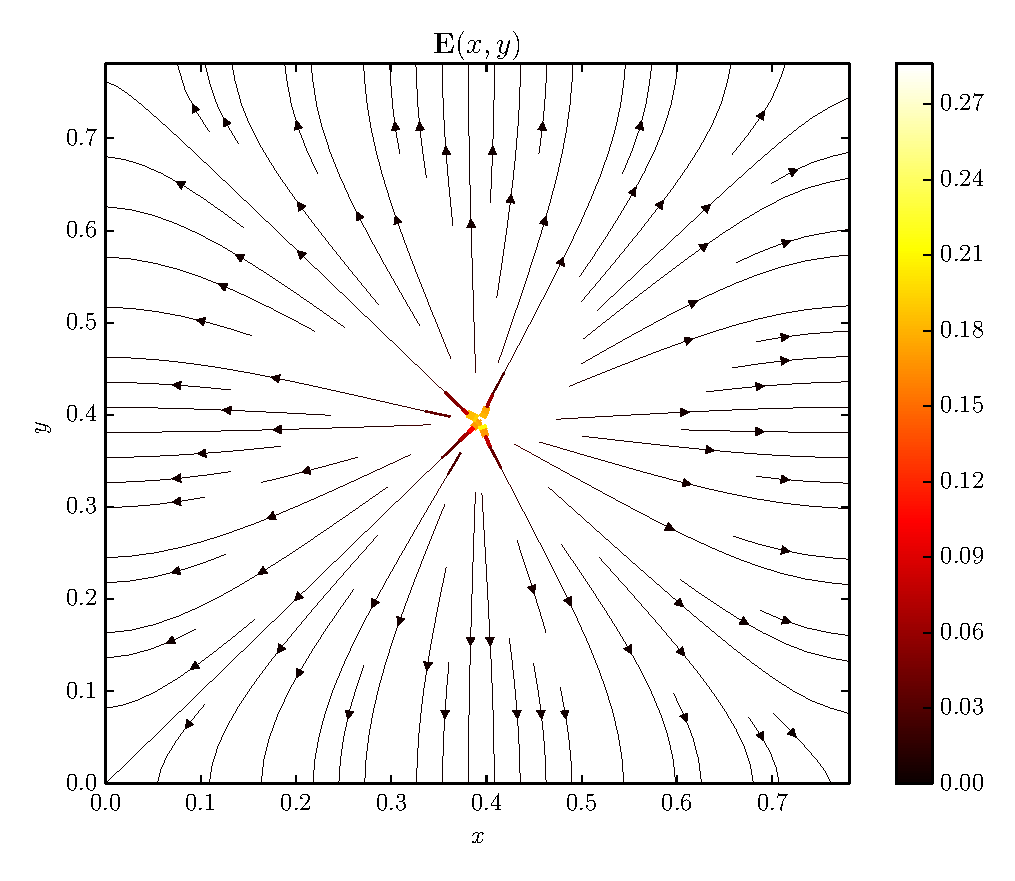
\includegraphics[width=0.3\linewidth]{graphs/examples/point_charge_vector.eps}
        \label{subfig:point_vect}
    }
    \caption{Plots of the solution to the Laplace equation for a single constant potential point.}
    \label{fig:point}
\end{figure}

\begin{figure}
    \centering
    \subfloat[Contour plot]{
        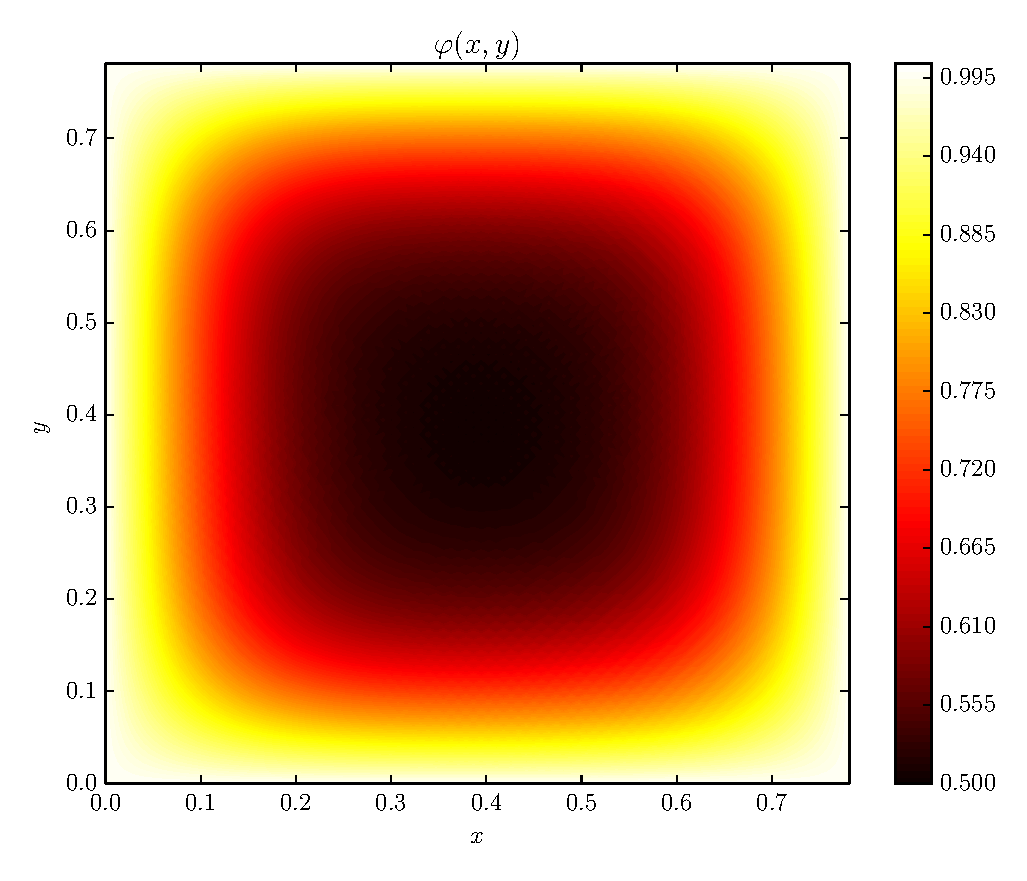
\includegraphics[width=0.3\linewidth]{graphs/examples/net_contour.eps}
        \label{subfig:net_cont}
    }
    \subfloat[Surface plot]{
        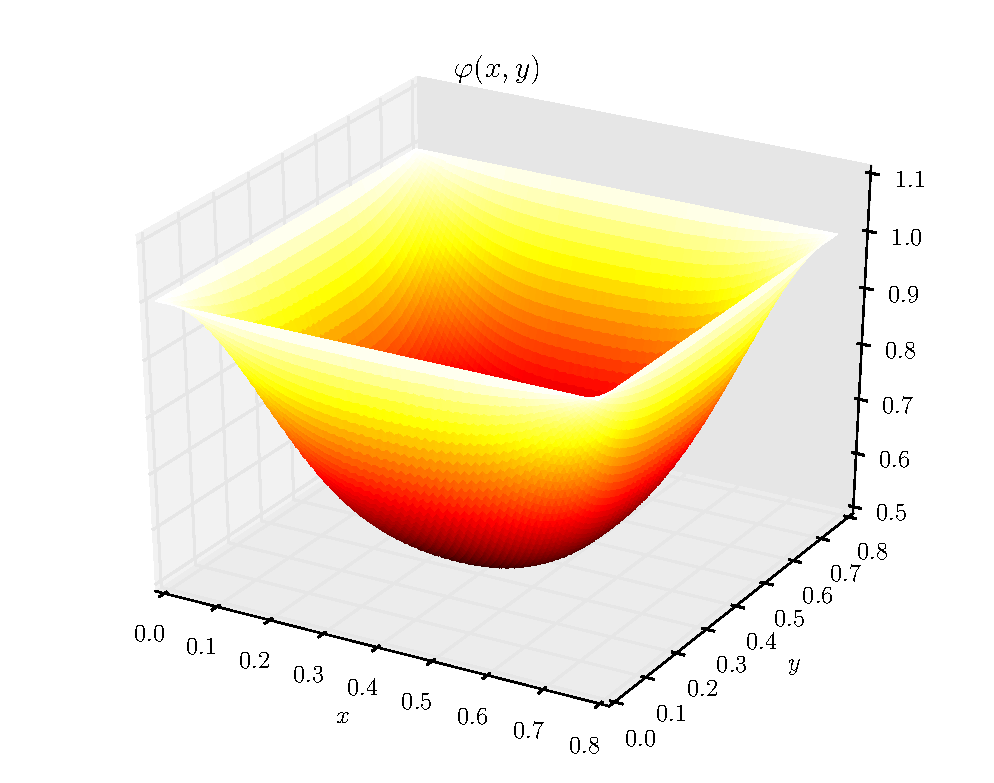
\includegraphics[width=0.3\linewidth]{graphs/examples/net_surf.eps}
        \label{subfig:net_surf}
    }
    \subfloat[Vector \textbf{E} field plot]{
        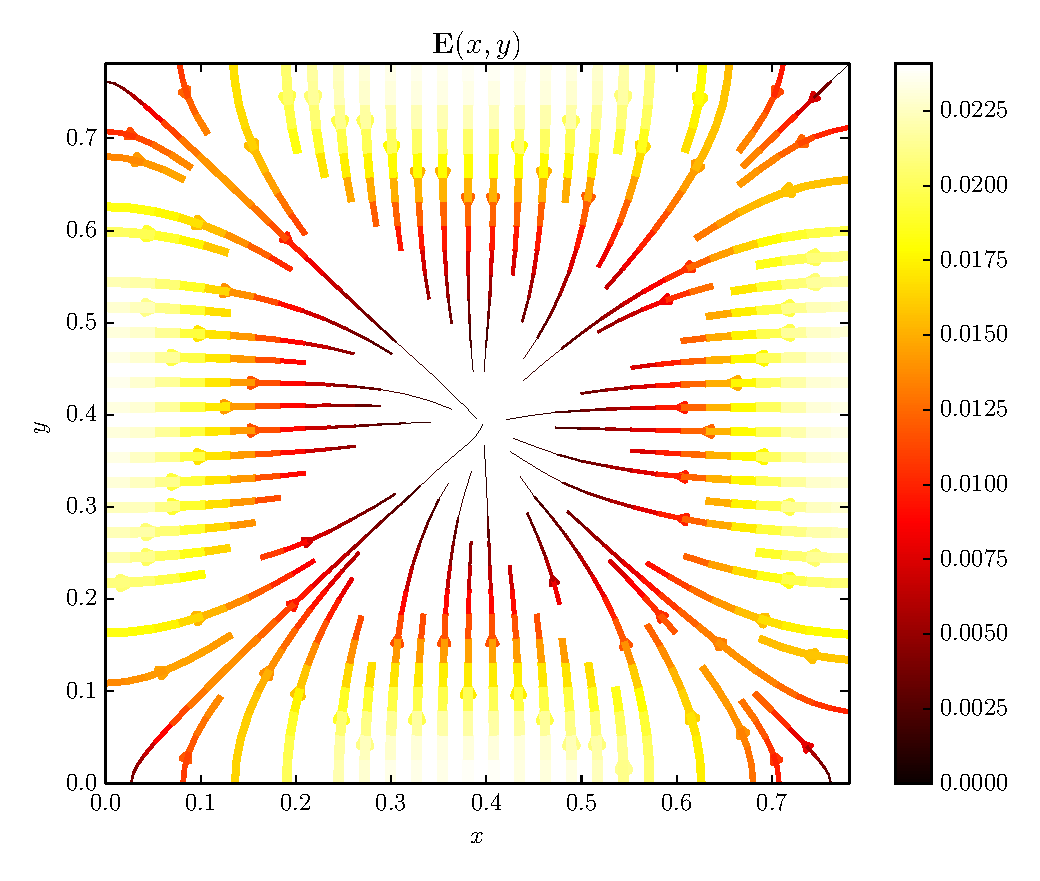
\includegraphics[width=0.3\linewidth]{graphs/examples/net_vector.eps}
        \label{subfig:net_vect}
    }
    \caption{Solution to the Laplace equation with edges of the grid held at constant positive potential.}
    \label{fig:net}
\end{figure}

\begin{figure}
    \centering
    \subfloat[Contour plot]{
        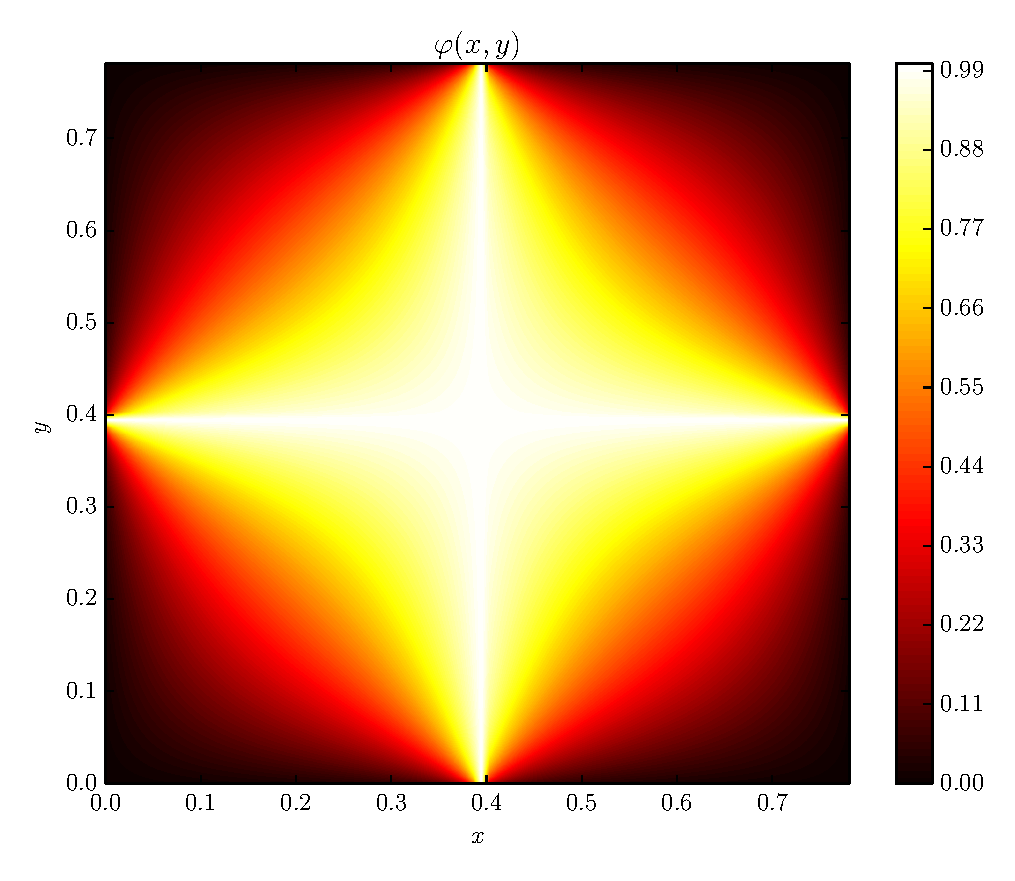
\includegraphics[width=0.3\linewidth]{graphs/examples/cross_contour.eps}
        \label{subfig:cross_cont}
    }
    \subfloat[Surface plot]{
        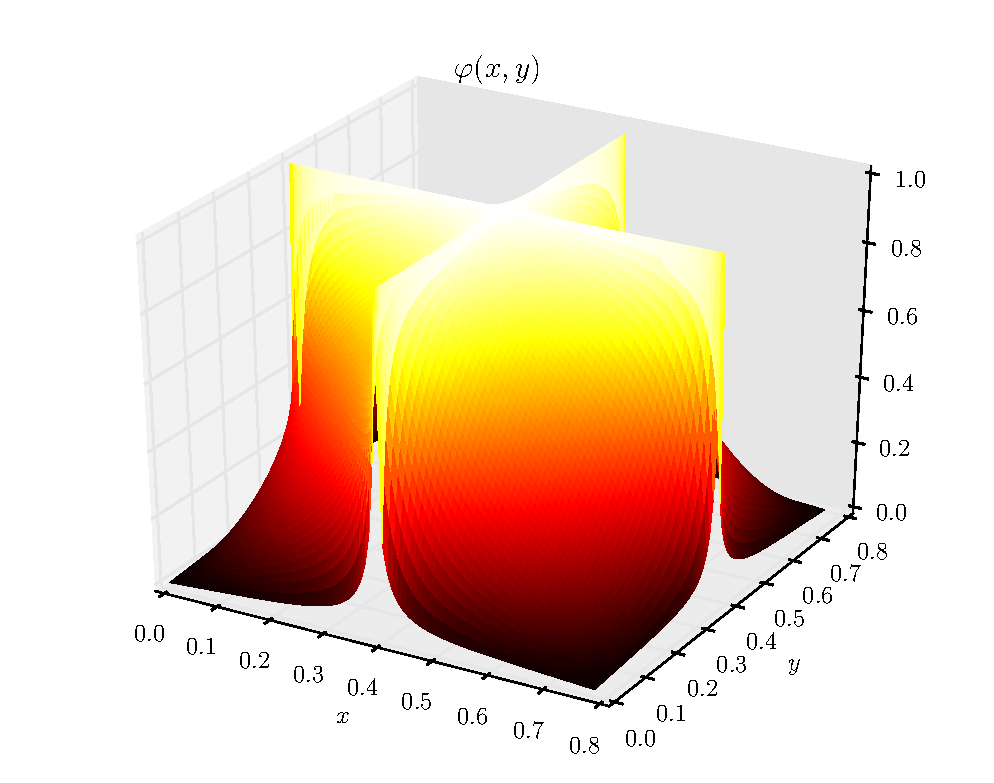
\includegraphics[width=0.3\linewidth]{graphs/examples/cross_surf.eps}
        \label{subfig:cross_surf}
    }
    \subfloat[Vector \textbf{E} field plot]{
        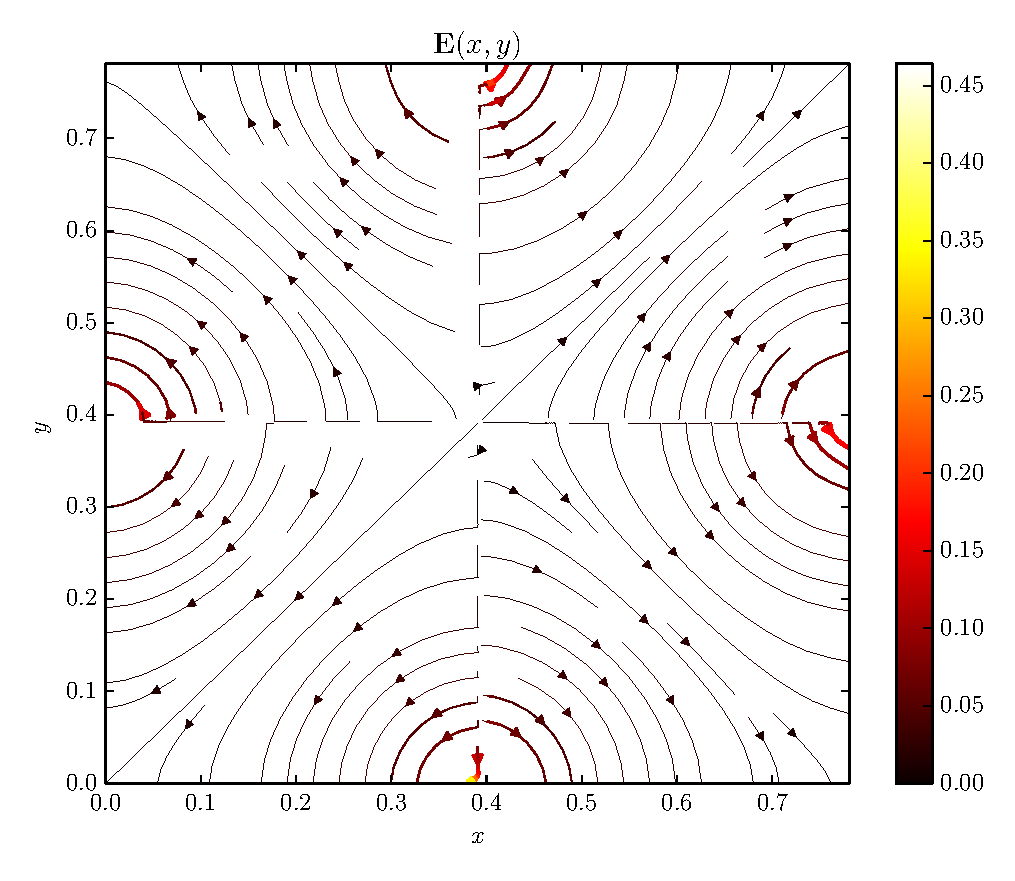
\includegraphics[width=0.3\linewidth]{graphs/examples/cross_vector.eps}
        \label{subfig:cross_vect}
    }
    \caption{Solution to the Laplace equation with equipotential cross overlaid on grid.}
    \label{fig:cross}
\end{figure}

\subsection{Convergence Condition}
\label{subsec:convergence_condition}

An absolute convergence condition is implemented to decide when the program has successfully iterated to the solution of the Laplace equation with the set boundary conditions. As compared to a relative convergence conditions, e.g. that no value changes by more than $X\%$, this has the disadvantage of depending on the boundary conditions applied to the system. So an absolute error tolerance of $\epsilon = \SI{0.01}{V}$ may be appropriate if the highest boundary condition is $\mathcal{O}(\SI{100}{V})$, but inappropriate if the potential boundary condition is $\mathcal{O}(\SI{0.1}{V})$. This is compensated for by the ability to manually change the error tolerance with the \texttt{--error} flag. By default this value is set at $10^{-4}$. When the boundary conditions are a single constant potential of \SI{1}{V} at the centre of the grid, the effect of a relatively large tolerance is to fatten the potential field around the point in the centre, as shown in Figure \ref{fig:tolerances}. This is because a too high $\epsilon$ means the iterations stop before a true solution is found. As there are no charges involved, the effect of each iteration is merely to average from the surrounding nodes. Hence when the program finishes the iterations early, it means it has prematurely ceased this averaging process and thus is higher near the central peak than it should physically be.

Increasing the absolute tolerance does, however, radically decrease the time taken and number of iterations needed to converge. Figure \ref{subfig:error_1e-2}, with $\epsilon = 10^{-2}$ on a grid of 100 by 100 took 95.56 seconds and 1815 iterations to converge, whilst Figure \ref{subfig:error_1e-6} took 784.33 seconds and 13789 iterations to converge. There is thus a trade off between time taken to converge and the precision of the convergent solution, as would be expected. Note that the average time taken per iteration, at 52.7 and 56.8 milliseconds for $\epsilon = 10^{-2}$ and $\epsilon = 10^{-6}$ respectively, is roughly unchanged.

\begin{figure}
    \centering
    \subfloat[$\epsilon = 10^{-2}$]{
        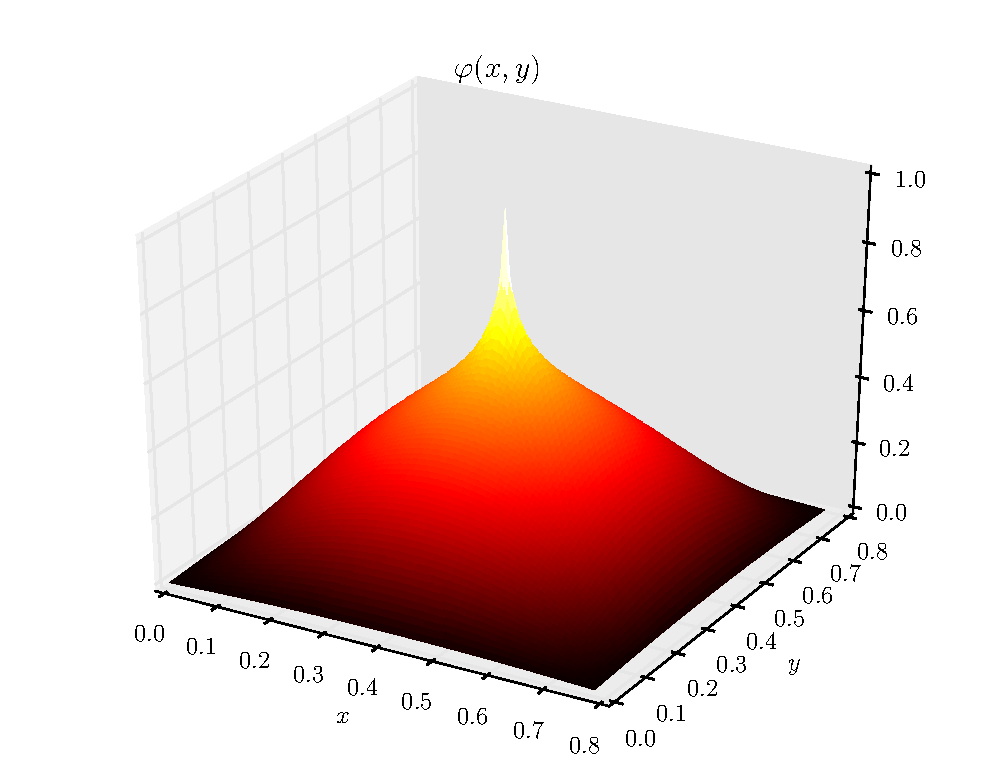
\includegraphics[width=0.5\linewidth]{graphs/tolerance/point_charge_error_1e-2_surf.eps}
        \label{subfig:error_1e-2}
    }
    \subfloat[$\epsilon = 10^{-6}$]{
        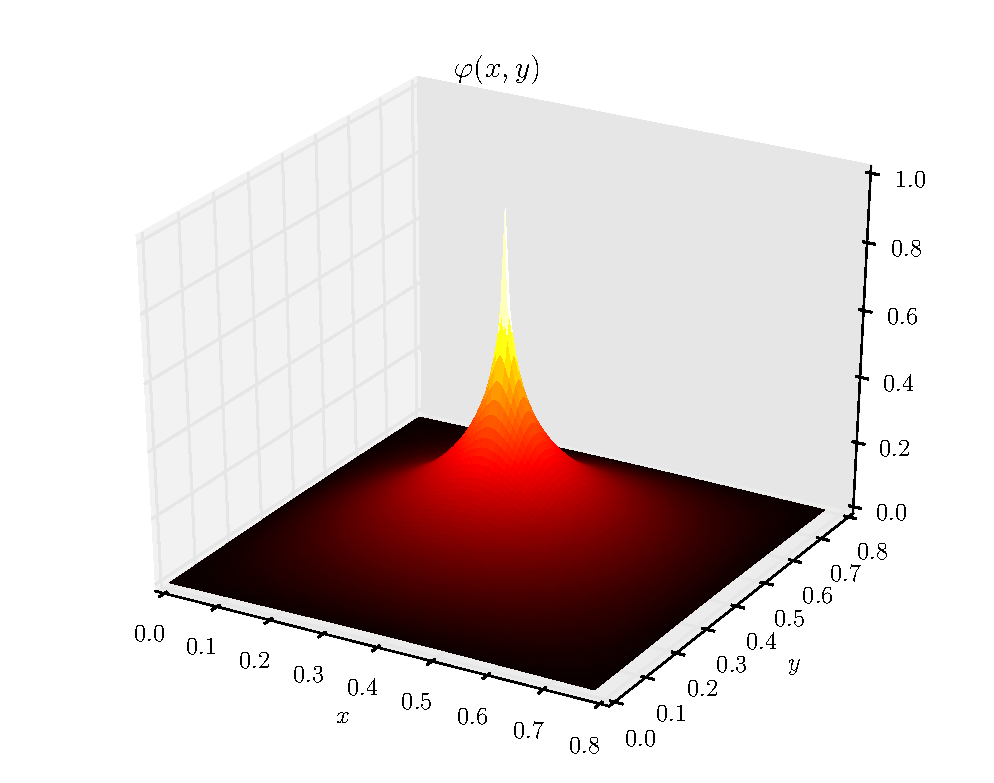
\includegraphics[width=0.5\linewidth]{graphs/tolerance/point_charge_error_1e-6_surf.eps}
        \label{subfig:error_1e-6}
    }
    \caption{Comparison of the effect of altering the absolute error tolerance, $\epsilon$, in the convergence condition on the resulting solution.}
    \label{fig:tolerances}
\end{figure}

\subsection{Iteration Method}
\label{subsec:iteration_method}

Both the Jacobi and Gauss-Seidel iteration methods are implemented, with the option of which to use left up to the user with the positional argument \texttt{method} determining which to use. Surprisingly, the Gauss-Seidel and Jacobi show no statistically significant changes in the time taken to converge or number of iterations needed to converge. When tested 20 times on a 100 by 100 grid, using the boundary conditions of the parallel plate capacitor as a test case, the Jacobi method averaged $313.78 \pm 63.39$ seconds of processor time and $4045 \pm 601$ iterations as compared to the Gauss-Seidel method, which took $319.23 \pm 55.27$ seconds and $4120 \pm 664$ iterations. Equally, when tested using different boundary conditions and grid densities, there consistently is no significant performance difference between the two. For a plane equipotential on a 32 by 32 grid averaging from 20 runs, Jacobi takes $2.94 \pm 0.28$ processor seconds and $537 \pm 48$ iterations, whilst Gauss-Seidel requires $3.00 \pm 0.34$ seconds and $555 \pm 61$ iterations, well within each others' standard error. This is contrary to popular presentations of the Gauss-Seidel method as the slightly faster of the two \cite{edwards2004,golub1996}, although no such general result can be said to hold \cite{demmel1997}. The two methods produce identical convergent results given the same input variables, as would be expected.
\subsection{Grid Density}
\label{subsec:grid_density}

The default parameters of the grid density are a 50 by 50 grid. Changing the density significantly increases the time taken to find a converging solution. In particular combining high density with very low tolerance results in extremely long convergence times, as shown by the fact that Figure \ref{subfig:error_1e-6} with a grid density of 100 by 100 and absolute error tolerance of $\epsilon = 10^{-6}$ took 784.33 processor seconds and 13789 iterations to converge, whilst with the much lower grid density of 32 by 32, again with $\epsilon = 10^{-6}$, convergence takes only 9.48 processor seconds and 1651 iterations, significantly lower. This also demonstrates that an increase in grid density significantly increases the processor time taken to run each iteration. For 100 by 100 grid with $\epsilon = 10^{-6}$, each iteration on average took 56.9 milliseconds, whilst for the 32 by 32 grid with $\epsilon = 10^{-6}$, each iteration took only 5.7 milliseconds. This means this increase in grid density resulted in an increase in the time taken to complete each iteration by a factor of ten. This implies that while the convergence condition affects the number of iterations needed to converge, it does not affect the time taken per iteration, whilst the grid density increases the time taken per iteration. This makes sense because the convergence condition only makes more stringent the requirement that classifies when the solution has been found and iterations can stop, whilst the grid density increases the number of nodes that need to be evaluated by finite difference for each iteration (which spans the whole grid).

\subsection{Grid Edges}
\label{subsec:grid_edges}

The problem arises when using the iteration formula given in Equation \ref{eqn:iteration} that when iterating at the edges of the grid, i.e. when grid indices $i=0$ or $j=0$, there are not four neighbouring nodes to include in the iteration. The approximation is made that these nodes outside of the grid can be taken as zero, as opposed to averaging over the neighbouring nodes that are within the grid. This is an acceptable approximation because it produces similar if not identical results and converges significantly faster. Figure \ref{fig:grid_edges} shows a comparison of the potential field around a constant potential point whilst making the assumption and without making the assumption (i.e. averaging over the nodes within the grid only). As can be seen, the two results are nearly identical, with the minor difference that Figure \ref{subfig:no_assume} has serrated grid edges. This is an artefact of the edges not having the full four neighbouring nodes to average from. However, the solution in Figure \ref{subfig:no_assume} took 218.92 seconds of processor time and 3908 iterations to converge, taken from an average of 10 runs, whilst \ref{subfig:assume} took only 26.42 processor seconds and 519 iterations, again from an average of 10 runs. These tests were done using the Gauss-Seidel iteration method. Given that this is a factor of 8 times faster, requiring 7.5 times fewer iterations to converge, to produce very similar results, the assumption is justifiable.

\begin{figure}
    \centering
    \subfloat[Making the assumption]{
        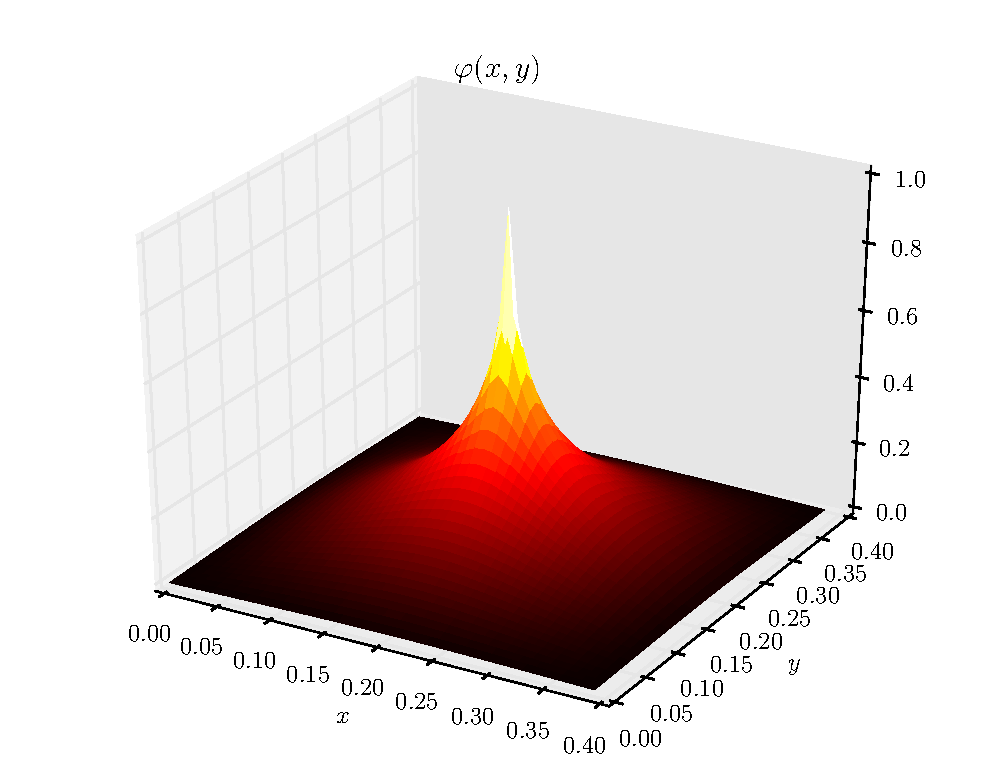
\includegraphics[width=0.5\linewidth]{graphs/grid_edges/assume_50x50_error_1e-4_surf.eps}
        \label{subfig:assume}
    }
    \subfloat[Without making the assumption]{
        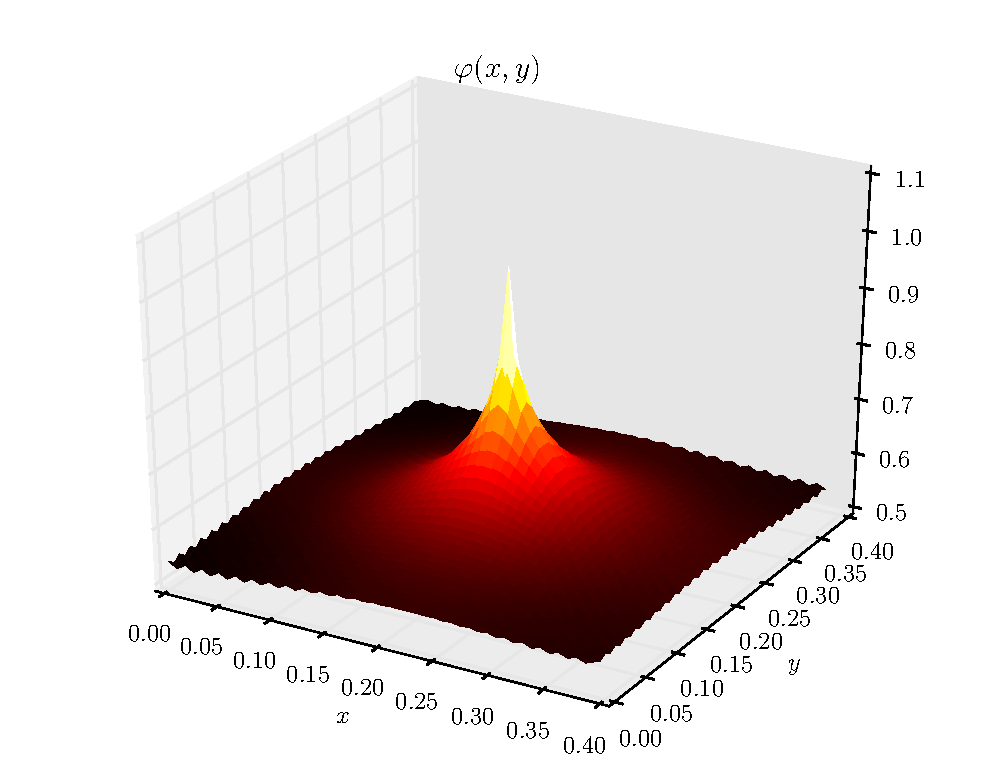
\includegraphics[width=0.5\linewidth]{graphs/grid_edges/no_assume_50x50_error_1e-2_surf.eps}
        \label{subfig:no_assume}
    }
    \caption{A comparison of the results produced by the Gauss-Seidel method when making the assumption that non-grid nodes are zero and without making the assumption.}
    \label{fig:grid_edges}
\end{figure}
